\chapter{Robot Quick start guide}
A big part of this was derived from \cite{MatlabControl}.

\paragraph{Parts of the robot}
A quick overview over the visible parts.

\subparagraph{FANUC R-2000iC/210F 6 axis robotic arm}
The robot has 6 movable joints with a possible payload attached to the end. Its features include a wide reach (2655 mm), sturdy but flexible arm design, a spring loaded counterbalance, relatively high payload capacity (210Kg) and fast moving axes. The joints also have hashes to indicate the zero positions which help with the calibration of the robot. 

\subparagraph{R30iA Robot Controller }
The Robot is controlled using an original equipment manufacturer controller called the FANUC R30iA controller. Its features include faster sustained speed and superior position accuracies. It also has the I/O ports that are used to connect grippers and other payloads. (It also houses the camera circuits which are required to access the data from the SONY camera provided with the robot. - Delta only)  The controller is also provided with a data card slot in which the special SD cards manufactured can be inserted and used as external memory. On the outside of the controller (side of iPendant at Delta) a USB port can be found. With these, programs, firmware files and other files can easily be transferred. Additionally, there is extended connectivity via its Ethernet port e.g. for FTP available.

\subparagraph{iPendant}
The teaching pendant is the primary user interface to the robot. It is used to move the joints of the robot manually, to program specific trajectories, to control the gripper, and various other actions. It also is an interface that can be used for input and output of the robot controller parameters. The user can access the system variables and position variables. (It is provided with a USB port that can be used to connect to a USB drive for external storage. - Delta only) It can also be used to setup an FTP server and client in order to communicate with the PC. 

\subparagraph{Gripper}
The robot as handed over does not have an active gripper system. It has been tested though with a pneumatic gripper controlled via the DO ports and pneumatic valves. A 2-way pneumatic valve, some piping and a pressure regulator are still available. (Delta Equipment varies here a lot).


\paragraph{iPendant Navigation Manual:}
The teaching pendant is the primary user interface to the robot. This section deals with the important 
buttons on the TP. 


\begin{figure}[H]
	\centering
	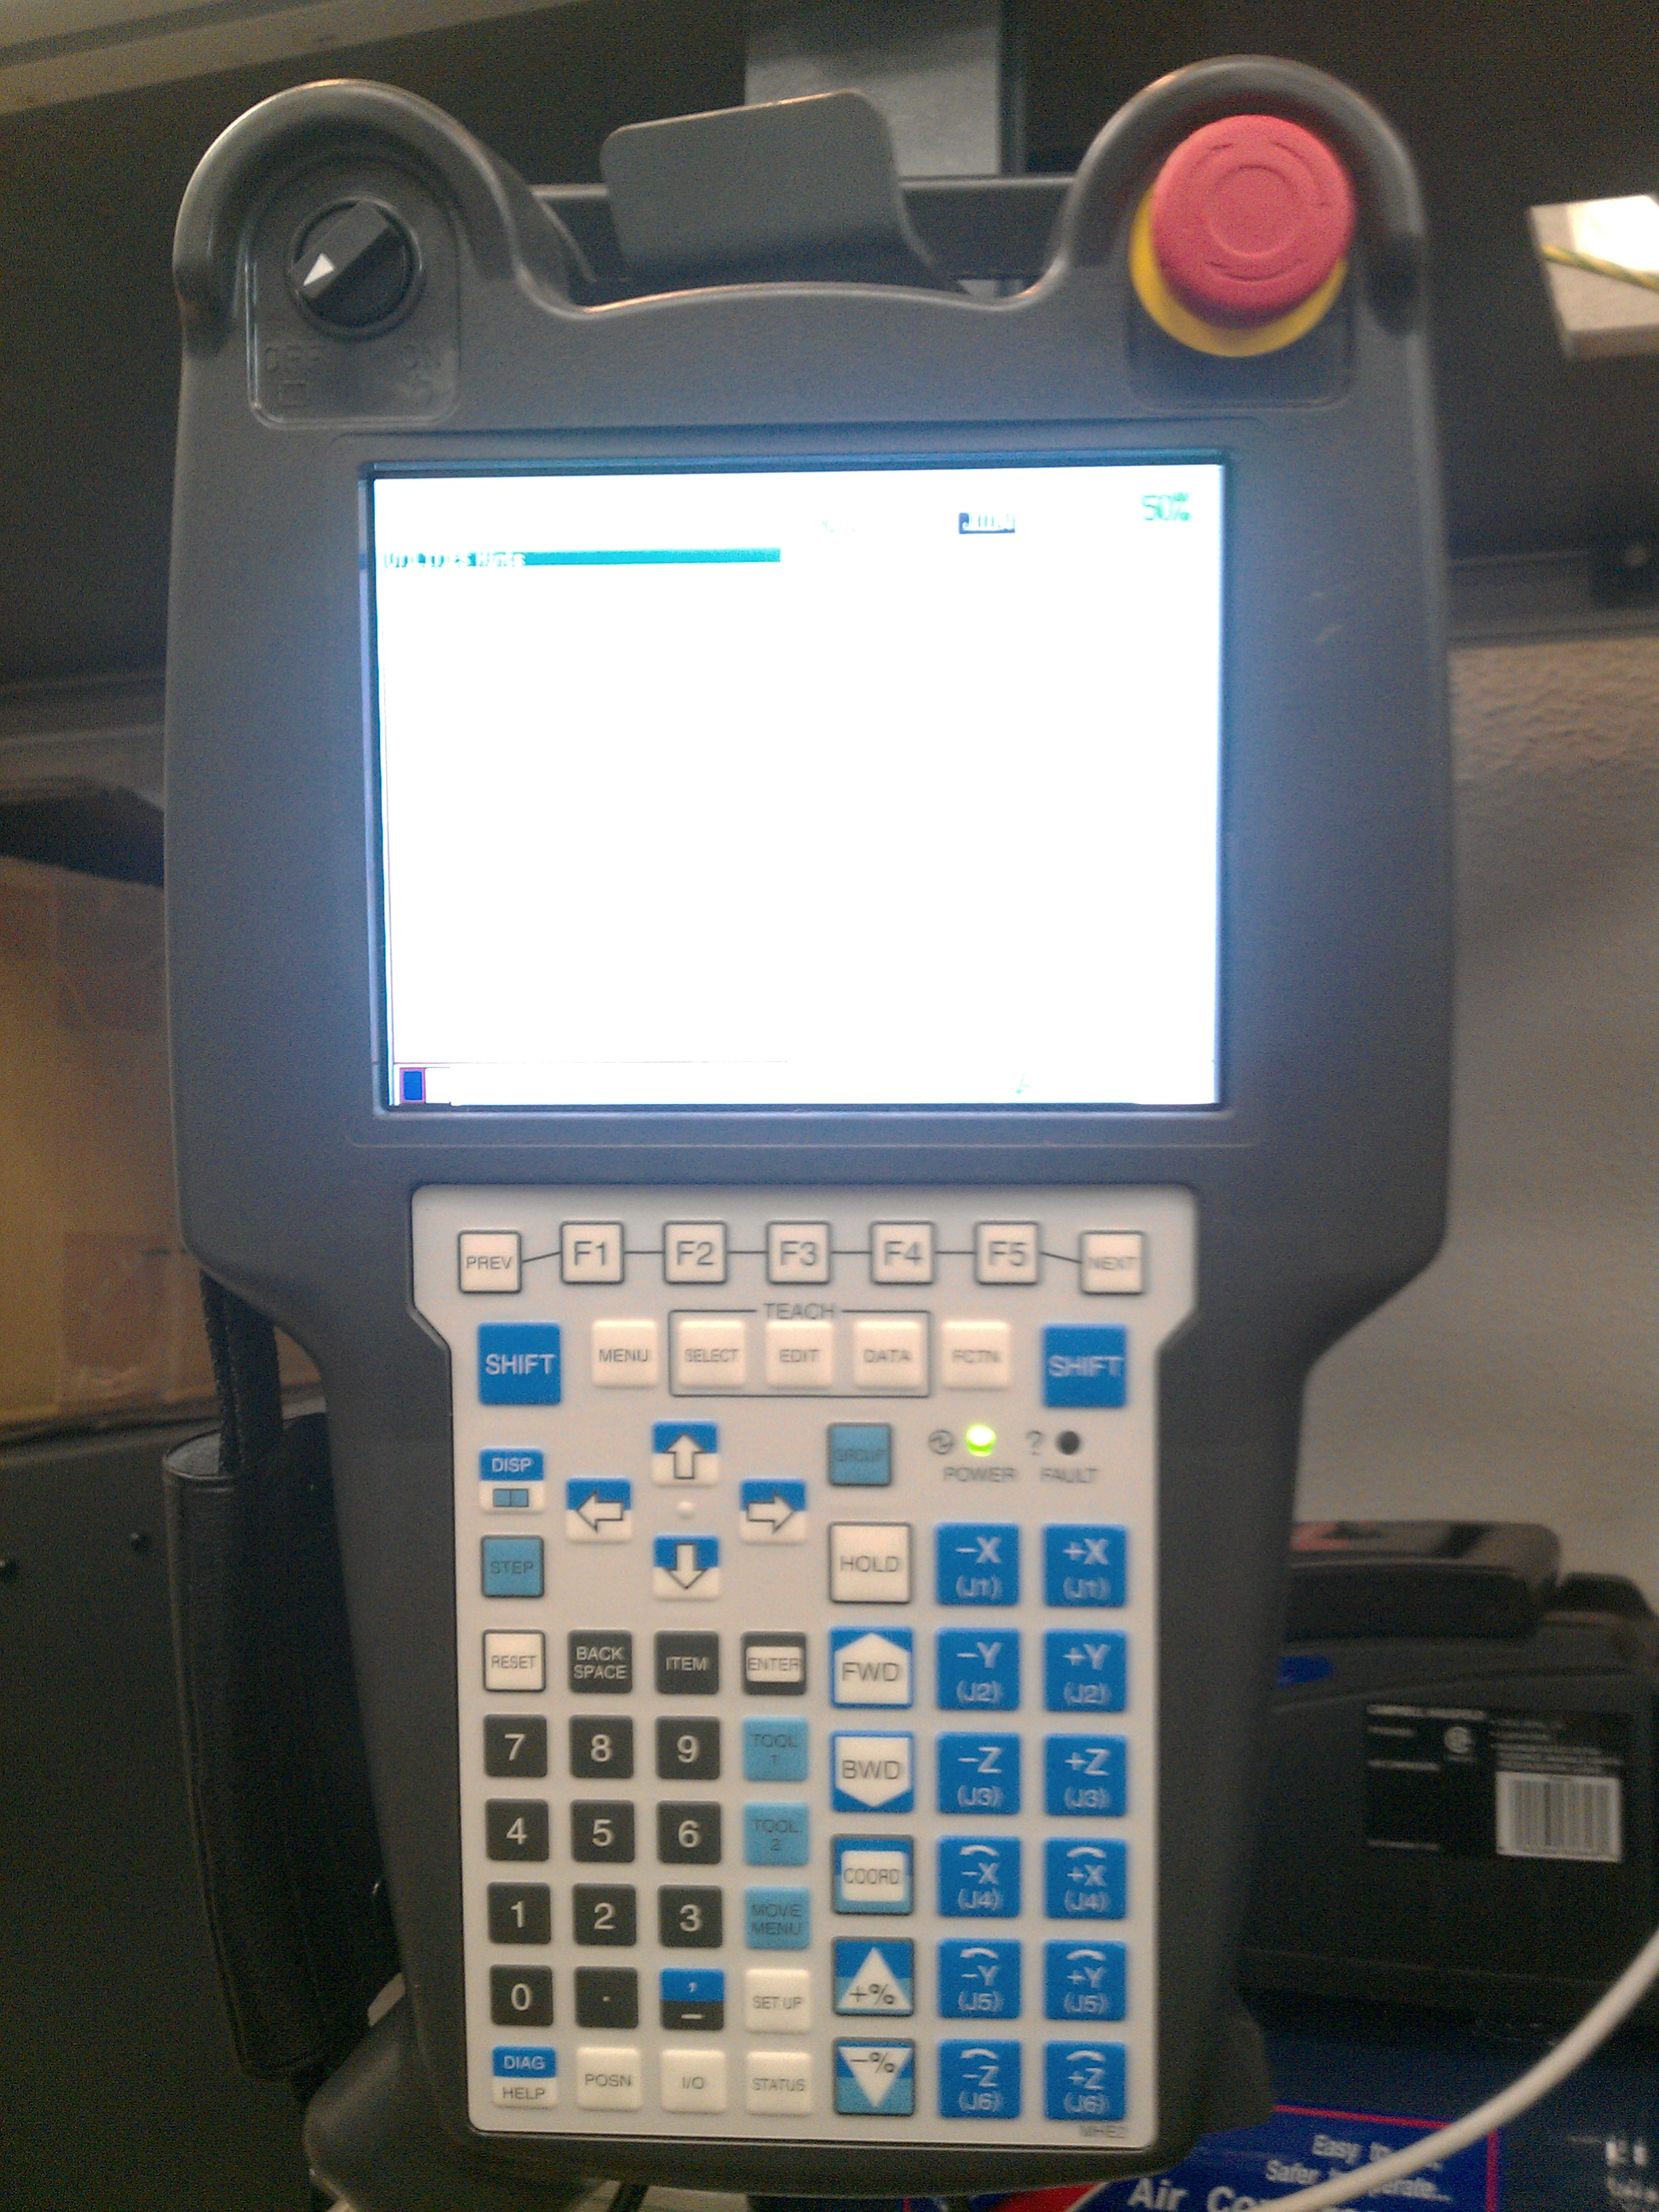
\includegraphics
	[width=0.8\linewidth
	]{images/iPendant_Numbered}
	\caption[Important buttons]{Most important iPendant buttons numbered: This image from another iPendant than the ones available was chosen because of its labelling of buttons. Some buttons of the available iPendants are not labelled, so this picture can be used as a reference. Source: \cite{MatlabControl}}
	\label{fig:ipendantnumbered}
\end{figure}


\subparagraph{Emergency stop: }

Makes the robot stop immediately by applying brakes. Use it only when necessary as the brakes wear down. There is also an E-stop on the controller.
Press down on the button to activate it.
Twist it to the right to release.
If a slow and gradual halt is required, press HOLD on the iPendant.
TP on/off:
Below the E-stop button. It should be ON to access any function in the Teach Pendant (Set-ups, calibration, programs etc) and OFF when running in AUTO mode.
Deadman switch
The 2 yellow bars behind the iPendant. 3 modes are available: Fully released, halfway pressed, fully pressed. Only the middle mode activates control.






